\chapter{Ball Tracking}
\label{ch:ball}

% Compact node styles for the TrackNet-family architecture schematics (Fig.~\ref{fig:ball-arch}).
\tikzset{
  tn/.style={rectangle, draw=blue!55, fill=blue!5, rounded corners,
    align=center, minimum height=0.85cm, text width=1.7cm,
    font=\scriptsize\sffamily, semithick},
  tnio/.style={tn, draw=gray!65, fill=gray!12},
  tnmod/.style={tn, draw=orange!80, fill=orange!15},
  tnarr/.style={-{Stealth[scale=0.9]}, line width=0.6pt, gray!70},
}

This chapter applies the protocol of Chapter~\ref{ch:methodology} to the first
and most demanding perception sub-task of the system, localising the tennis
ball in every frame. The ball is small, often blurred by its own speed, and
regularly hidden by players, the net, or the court markings, so its position
must be inferred from motion across several frames rather than from any single
image. Six models are compared: the five published members of the TrackNet
family, V1 through V5, and a single-frame object detector, YOLO11m, included as
a representative of the bounding-box paradigm against which the heatmap
formulation is contrasted. All six operate on the TrackNet tennis dataset
described in Section~\ref{sec:meth-tracknet} and are scored by the localisation
and detection metrics of Sections~\ref{sec:meth-metrics-loc}
and~\ref{sec:meth-metrics-det}.

The comparison follows a deliberate two-stage selection protocol, which shapes
how the results in Sections~\ref{sec:ball-selection}
and~\ref{sec:ball-final} should be read. In the first stage, architecture
selection, all six models were trained and evaluated on a smaller subset split
in order to compare the architectures cheaply. In the second stage, the single
winner of that comparison, TrackNetV4, was retrained on the full dataset split
defined in Section~\ref{sec:meth-splits-tracknet}. The two stages therefore
report different numbers measured on different held-out matches, and a figure
from one stage is never placed beside a figure from the other without that
distinction being made explicit. This design is a defensible compromise between
rigour and cost: it compares six architectures on a common footing, then
invests full-dataset training only in the chosen one, and it is the structure
through which the chapter answers the first research question (RQ1) on which
architecture best localises the ball and what the architectural progression
buys in accuracy against speed.

\section{Task Formulation}
\label{sec:ball-task}

Ball tracking is posed here as per-frame localisation rather than as
multi-object tracking. For each frame the model must report either a single
image coordinate for the ball or an explicit indication that no ball is
present, and the per-frame outputs are read as a trajectory without an explicit
data-association stage. Two formulations of this task are compared. In the
heatmap formulation, which the TrackNet family adopts, the network predicts a
spatial response map whose peak marks the ball centre, and the coordinate is
recovered by locating the maximum response; the absence of a ball is expressed
naturally as a map with no significant peak \cite{huang2019tracknet,
zhou2019centernet}. In the bounding-box formulation, which the YOLO detector
adopts, the network regresses a box around the ball and its centre is taken as
the position, with a confidence score gating whether a ball is reported at all
\cite{redmon2016yolo}. The contrast between these two formulations on a small,
fast, frequently occluded target is the central question of the chapter, and
the absence of a ball is represented throughout by the coordinate $(-1, -1)$,
the sentinel defined in Section~\ref{sec:meth-tracknet}.

\section{Preprocessing and Learning Targets}
\label{sec:ball-preproc}

The temporal cue that distinguishes a moving ball from the static background is
provided to the models by stacking consecutive frames. For the TrackNet family
a sliding window of three consecutive frames is read from a clip and stacked
along the channel axis into a nine-channel input, with the ball position of the
middle frame as the target; the first and last frames of every clip are skipped
so that a complete window of three frames is always available. The frames are
resized before stacking, and the resize convention differs by model and by
stage. In the architecture-selection comparison of
Section~\ref{sec:ball-selection}, V1, V4, and V5 operate on a square
$256 \times 256$ input, V2 and V3 at $512 \times 288$, and the YOLO detector at
its native $640 \times 640$; the final TrackNetV4 of
Section~\ref{sec:ball-final} was retrained at the higher $640 \times 368$
resolution, which preserves the broadcast aspect ratio rather than squashing it
to a square. These conventions are not
intermixed, and every coordinate reported by a model is both expressed and
scored in its own resized pixel space rather than being rescaled to a common
frame.

The learning target depends on how each model represents the ball. The original
V1 design and its V4 descendant do not regress a continuous heatmap but instead
predict a quantised intensity class map: a Gaussian centred on the ball, of
half-size 20 pixels and variance 10, is rendered and quantised so that each
pixel carries an integer intensity class in the range $[0, 255]$, with the peak
value 255 at the ball centre, and the network is trained to classify every
pixel into one of these 256 classes. V2 and V3 instead regress a continuous
Gaussian heatmap with a sigmoid output and a peak value of one, as does V5. The
YOLO detector is trained against a fixed bounding box of 20 pixels placed around
the labelled point, in the YOLO annotation format. In all cases a frame whose
ball is invisible (visibility class~0, or a blank or negative coordinate)
produces an all-zero target and contributes the $(-1, -1)$ sentinel rather than
a spurious position.

Data augmentation is applied to the training split only, with validation and
test frames left unaltered. The augmentation perturbs brightness by up to
$\pm 0.3$ of the intensity range and scales contrast by a factor drawn from
$[0.7, 1.3]$, and with probability one half it flips the frame window
horizontally. The flip is the one augmentation that interacts with the label:
when a window is flipped, the ball x-coordinate is remapped to $W - 1 - x$,
where $W$ is the frame width, so that the target stays aligned with the
image, while an invisible ball (coordinate $-1$) is left untouched. The same
transformation is applied consistently across all three frames of a window so
that the temporal cue is preserved.

\section{Models}
\label{sec:ball-models}

The five TrackNet variants share a common lineage, an encoder-decoder
convolutional network with skip connections that ingests the nine-channel frame
stack and produces a spatial output at the input resolution
\cite{huang2019tracknet}. They differ in the output representation, in the depth
of the encoder-decoder, and in the temporal-reasoning module each one adds.
Table~\ref{tab:ball-models} summarises the six models along the axes that
matter for the comparison, and the architecture of each of the five TrackNet
variants is drawn in Figure~\ref{fig:ball-arch}, panels (a) to (e).

\begin{table}[t]
  \centering
  \small
  \setlength{\tabcolsep}{4pt}
  \caption{The six ball-tracking models compared in this chapter. The TrackNet
    family shares an encoder-decoder backbone and differs in its output
    representation and temporal module; YOLO11m is a single-frame bounding-box
    detector included as the non-heatmap baseline. Parameter counts are computed
    from the implementations used here; the YOLO11m figure is the published size
    of the Ultralytics medium model \cite{jocher2024yolo11}.}
  \label{tab:ball-models}
  \begin{tabular}{@{}l >{\raggedright\arraybackslash}p{3.0cm} >{\raggedright\arraybackslash}p{4.8cm} r@{}}
    \toprule
    Model & Output target  & Distinctive module & \makecell[r]{Params\\(M)} \\
    \midrule
    TrackNet (V1) & 256-class intensity map  & VGG encoder-decoder & 20.9 \\
    TrackNetV2    & multi-frame heatmaps      & multiple-in multiple-out & 11.3 \\
    TrackNetV3    & multi-frame heatmaps      & median background + InpaintNet & 11.3 \\
    TrackNetV4    & 256-class intensity map & motion-attention gating & 20.9 \\
    TrackNetV5    & single heatmap          & temporal self-attention & 21.9 \\
    YOLO11m       & bounding box            & anchor-free box regression & 20.1 \\
    \bottomrule
  \end{tabular}
\end{table}

TrackNet (V1), in panel~(a), follows the original design
\cite{huang2019tracknet}: a
four-stage VGG-style encoder with max-pooling, a convolutional bottleneck, and a
symmetric decoder whose transposed convolutions are concatenated with the
matching encoder features through skip connections. A final $1 \times 1$
convolution maps the decoded features to 256 channels, one per intensity class,
and the position is recovered by taking the per-pixel argmax to form an
intensity image and locating its global peak; a peak below an intensity
threshold yields the no-ball sentinel. This is a multiple-in single-out design,
three frames in and one ball position out.

TrackNetV2, in panel~(b), reorganises the backbone into a multiple-in
multiple-out form that predicts a sigmoid Gaussian heatmap for every frame in
the window in a single pass, reducing redundant computation
\cite{sun2020tracknetv2}. Its
encoder-decoder is shallower than V1's, three stages rather than four, with
nearest-neighbour upsampling in the decoder, which roughly halves the parameter
count to 11.3~million. The coordinate is the argmax of the relevant frame's
heatmap when its peak exceeds 0.5, and the sentinel otherwise.

TrackNetV3, in panel~(c), builds on the V2 backbone with two additions
aimed at robustness \cite{chen2023tracknetv3}. A per-pixel median-background channel,
computed across the input window, is concatenated to the frame stack so that the
network sees an explicit estimate of the static scene. Separately, an
inpainting network, a small one-dimensional U-Net that takes a sequence of
predicted coordinates with a visibility flag and outputs a rectified sequence,
repairs missed detections by reasoning over the predicted path; it is trained
with a mean-squared-error objective on the trajectory and operates as a
post-processing stage over the tracker's per-frame peaks.

TrackNetV4, in panel~(d), is the model selected in
Section~\ref{sec:ball-selection}. It keeps the V1 backbone and
256-class output, and adds a lightweight motion-attention module
\cite{raj2025tracknetv4}. The module forms absolute differences between
successive input frames, passes the concatenated difference maps through two
convolutions and a sigmoid to produce a single-channel spatial attention map,
and multiplies this map into the decoder features at two resolutions. The effect
is to amplify regions of recent motion, where a fast ball is likely to be, while
suppressing the static background, at a negligible parameter cost over V1
(20.9~million for both).

TrackNetV5, in panel~(e), encodes each of the three frames independently
with a shared
VGG-style encoder, then fuses their deepest features with a multi-head temporal
self-attention layer that treats the three frames as a short sequence at each
spatial position, before decoding from the attended middle-frame features to a
single sigmoid heatmap. It is the largest of the family at 21.9~million
parameters. As noted in Section~\ref{sec:rw-tracknet}, V5 is a preprint variant
\cite{tang2025tracknetv5} and is included to test whether learned temporal
attention improves on the explicit motion cue of V4.

YOLO11m is a single-frame, anchor-free object detector from the
Ultralytics YOLO family \cite{jocher2024yolo11, redmon2016yolo}. Unlike the
TrackNet models it sees one frame at a time and regresses a bounding box whose
centre is taken as the ball position, with a confidence threshold of 0.3 below
which no ball is reported. It carries no temporal cue and serves as the
bounding-box baseline against which the heatmap formulation is measured.

\begin{figure}[p]
  \centering
  \begin{subfigure}{\textwidth}
    \centering
    \resizebox{\textwidth}{!}{%
    \begin{tikzpicture}[node distance=0.4cm and 0.6cm]
      \node[tnio] (i) {3 frames\\(9 ch)};
      \node[tn, right=of i] (e) {encoder\\4 stages};
      \node[tn, right=of e] (b) {bottleneck};
      \node[tn, right=of b] (d) {decoder\\+ skips};
      \node[tn, right=of d] (h) {256-class\\head};
      \node[tnio, right=of h] (o) {$\arg\max$\\$\to (x,y)$};
      \foreach \x/\y in {i/e,e/b,b/d,d/h,h/o} \draw[tnarr] (\x) -- (\y);
    \end{tikzpicture}}
    \caption{TrackNet (V1): four-stage VGG encoder-decoder with skip
      connections and a 256-class intensity head; multiple-in, single-out.}
    \label{fig:arch-v1}
  \end{subfigure}

  \vspace{0.8em}
  \begin{subfigure}{\textwidth}
    \centering
    \resizebox{\textwidth}{!}{%
    \begin{tikzpicture}[node distance=0.4cm and 0.6cm]
      \node[tnio] (i) {3 frames\\(9 ch)};
      \node[tn, right=of i] (e) {encoder\\3 stages};
      \node[tn, right=of e] (b) {bottleneck};
      \node[tn, right=of b] (d) {decoder\\+ skips\\(NN up)};
      \node[tn, right=of d] (h) {3 heatmaps\\(MIMO)};
      \node[tnio, right=of h] (o) {$\arg\max$\\$\to (x,y)$};
      \foreach \x/\y in {i/e,e/b,b/d,d/h,h/o} \draw[tnarr] (\x) -- (\y);
    \end{tikzpicture}}
    \caption{TrackNetV2: shallower three-stage backbone that emits one heatmap
      per input frame in a single multiple-in multiple-out pass.}
    \label{fig:arch-v2}
  \end{subfigure}

  \vspace{0.8em}
  \begin{subfigure}{\textwidth}
    \centering
    \resizebox{\textwidth}{!}{%
    \begin{tikzpicture}[node distance=0.4cm and 0.6cm]
      \node[tnio] (i) {frames +\\median bg\\(27 ch)};
      \node[tn, right=of i] (bb) {V2 backbone\\(MIMO)};
      \node[tn, right=of bb] (hm) {per-frame\\heatmaps};
      \node[tn, right=of hm] (p) {peak\\coords};
      \node[tnmod, right=of p] (ip) {InpaintNet\\1D U-Net};
      \node[tnio, right=of ip] (o) {rectified\\trajectory};
      \foreach \x/\y in {i/bb,bb/hm,hm/p,p/ip,ip/o} \draw[tnarr] (\x) -- (\y);
    \end{tikzpicture}}
    \caption{TrackNetV3: the V2 tracker fed an extra median-background channel,
      followed by an InpaintNet that rectifies the trajectory (shaded).}
    \label{fig:arch-v3}
  \end{subfigure}

  \vspace{0.8em}
  \begin{subfigure}{\textwidth}
    \centering
    \resizebox{\textwidth}{!}{%
    \begin{tikzpicture}[node distance=0.5cm and 0.6cm]
      \node[tnio] (i) {3 frames\\(9 ch)};
      \node[tn, right=of i] (e) {encoder};
      \node[tn, right=of e] (b) {bottleneck};
      \node[tn, right=of b] (d) {decoder\\+ skips};
      \node[tn, right=of d] (h) {256-class\\head};
      \node[tnio, right=of h] (o) {$\arg\max$\\$\to (x,y)$};
      \node[tnmod, below=0.7cm of b] (m) {motion\\attention};
      \foreach \x/\y in {i/e,e/b,b/d,d/h,h/o} \draw[tnarr] (\x) -- (\y);
      \draw[tnarr] (i.south) |- (m.west);
      \draw[tnarr] (m.east) -| (d.south);
    \end{tikzpicture}}
    \caption{TrackNetV4: the V1 backbone with a motion-attention branch (shaded)
      that gates the decoder towards moving regions; the selected model.}
    \label{fig:arch-v4}
  \end{subfigure}

  \vspace{0.8em}
  \begin{subfigure}{\textwidth}
    \centering
    \resizebox{\textwidth}{!}{%
    \begin{tikzpicture}[node distance=0.4cm and 0.55cm]
      \node[tnio] (i) {3 frames\\(per frame)};
      \node[tn, right=of i] (e) {shared\\encoder};
      \node[tn, right=of e] (b) {bottleneck\\feats $\times 3$};
      \node[tnmod, right=of b] (a) {temporal\\self-attn.};
      \node[tn, right=of a] (d) {decode\\middle};
      \node[tn, right=of d] (h) {heatmap};
      \node[tnio, right=of h] (o) {$\arg\max$\\$\to (x,y)$};
      \foreach \x/\y in {i/e,e/b,b/a,a/d,d/h,h/o} \draw[tnarr] (\x) -- (\y);
    \end{tikzpicture}}
    \caption{TrackNetV5: each frame is encoded independently and the three
      bottleneck features are fused by temporal self-attention (shaded) before
      decoding the middle frame.}
    \label{fig:arch-v5}
  \end{subfigure}

  \caption{Architecture of the five TrackNet-family variants compared in this
    chapter. All share an encoder-decoder backbone that ingests stacked frames
    and produces a spatial output decoded to a ball coordinate; they differ in
    the output representation and in the temporal module each one adds, shaded
    for the trajectory rectifier of V3, the motion attention of V4, and the
    temporal self-attention of V5.}
  \label{fig:ball-arch}
\end{figure}

\section{Training Details}
\label{sec:ball-training}

All models were trained on a single GPU with a learning-rate schedule that
reduced the rate by half when the validation loss plateaued, and with early
stopping that halted training when the validation accuracy at five pixels failed
to improve for a fixed number of epochs. Within this common regime the models
differ in optimiser, loss, and the hyperparameters listed in
Table~\ref{tab:ball-train}. The two 256-class models, V1 and V4, were trained
with the Adadelta optimiser and a cross-entropy loss over the intensity classes;
the heatmap-regressing V2 and V3 trackers used the Adam optimiser
\cite{kingma2015adam} with a weighted binary cross-entropy that emphasises the
sparse positive pixels in the manner of focal loss \cite{lin2017focalloss}; V5
used Adam with a plain binary cross-entropy on its sigmoid heatmap; and the
InpaintNet rectifier of V3 was trained separately with mean-squared error on the
coordinate sequence. YOLO11m was trained through the Ultralytics framework with
its own composite detection loss and optimiser defaults. The differences in
batch size and epoch budget in Table~\ref{tab:ball-train} reflect the differing
memory footprints and convergence behaviour of the models rather than a tuned
search, and every model was trained under the identical subset split of
Section~\ref{sec:ball-selection} so that the comparison is like-for-like.

\begin{table}[t]
  \centering
  \small
  \setlength{\tabcolsep}{6pt}
  \caption{Training configuration of the six models. All used a
    reduce-on-plateau learning-rate schedule and early stopping; they differ in
    optimiser, loss, and budget. The two 256-class models (V1, V4) use Adadelta
    with cross-entropy; the heatmap models use Adam.}
  \label{tab:ball-train}
  \begin{tabular}{l l l r r r}
    \toprule
    Model & Optimiser & Loss & \makecell[r]{Init.\\LR} & Batch & Epochs \\
    \midrule
    TrackNet (V1) & Adadelta & cross-entropy        & 1.0   & 4  & 50 \\
    TrackNetV2    & Adam     & weighted BCE         & $10^{-3}$ & 10 & 30 \\
    TrackNetV3    & Adam     & weighted BCE / MSE   & $10^{-3}$ & 10 & 30 \\
    TrackNetV4    & Adadelta & cross-entropy        & 1.0   & 4  & 50 \\
    TrackNetV5    & Adam     & BCE                  & $5\times10^{-5}$ & 8  & 60 \\
    YOLO11m       & SGD      & detection loss       & $10^{-4}$ & 16 & 50 \\
    \bottomrule
  \end{tabular}
\end{table}

\section{Model Selection: the Six Model Subset Comparison}
\label{sec:ball-selection}

The first stage of the protocol compared all six models on a subset split small
enough to train every architecture at modest cost. Matches game1 and game2 were
partitioned by clip into 70\% training, 15\% validation, and 15\% test
fractions, and game7 was held out in its entirety as an unseen-match test set on
which the comparison metrics were measured. This subset split is distinct from
the full split used for the final model in Section~\ref{sec:ball-final}: it
trains on far fewer matches and reports on a different held-out match (game7
rather than game10), so its numbers must be read as an internally consistent
ranking of architectures, not as the system's final accuracy. The results are
given in Table~\ref{tab:ball-selection}.

\begin{table}[t]
  \centering
  \footnotesize
  \setlength{\tabcolsep}{4pt}
  \caption{Six-model comparison on the subset test match (game7). All figures
    are measured on the same held-out match under one protocol; in particular
    every frames-per-second figure in this table was timed on the same GPU and
    is internally comparable, but is \emph{not} comparable with the final-model
    throughput of Table~\ref{tab:ball-final}, which was measured on different
    hardware (Section~\ref{sec:ball-final}). Bold marks the best value in each
    column; lower is better for $\mathrm{MAE_{px}}$ and tracking consistency
    (TC). The detection columns Prec, Rec, and $F_1$ are the visibility-based
    detection metrics of Section~\ref{sec:meth-metrics-det}, scoring only
    whether a ball is reported when one is in fact present; they are therefore
    distinct from the localisation accuracy $\mathrm{acc@}\tau$px and from the
    stricter location-aware precision@5px, recall@5px, and $F_1$@5px, which
    additionally require the prediction to fall within five pixels and are
    reported for the final model in Table~\ref{tab:ball-final}.}
  \label{tab:ball-selection}
  \begin{tabular}{l rrr r rrr r r}
    \toprule
    & \multicolumn{4}{c}{Localisation} & \multicolumn{3}{c}{Detection (visibility)} & & \\
    \cmidrule(lr){2-5} \cmidrule(lr){6-8}
    Model & \makecell[r]{acc@\\5px} & \makecell[r]{acc@\\10px} & \makecell[r]{acc@\\20px}
          & \makecell[r]{$\mathrm{MAE_{px}}$} & Prec & Rec & $F_1$
          & \makecell[r]{TC} & FPS \\
    \midrule
    TrackNet (V1) & 0.847 & 0.877 & 0.898 & \textbf{14.65} & 0.968 & 0.966 & 0.967 & 13.98 & \textbf{55.45} \\
    TrackNetV2    & 0.723 & 0.797 & 0.815 & 133.22 & \textbf{0.998} & 0.831 & 0.907 & 25.99 & 18.02 \\
    TrackNetV3    & 0.620 & 0.731 & 0.771 & 43.99 & 0.958 & \textbf{0.997} & \textbf{0.977} & 34.85 & 13.73 \\
    \textbf{TrackNetV4} & \textbf{0.875} & \textbf{0.895} & \textbf{0.905} & 15.20 & 0.982 & 0.937 & 0.959 & \textbf{10.44} & 53.07 \\
    TrackNetV5    & 0.720 & 0.737 & 0.752 & 35.70 & 0.978 & 0.852 & 0.911 & 13.31 & 26.04 \\
    YOLO11m       & 0.548 & 0.595 & 0.620 & 165.93 & 0.954 & 0.930 & 0.942 & 74.79 & 47.68 \\
    \bottomrule
  \end{tabular}
\end{table}

Tracking consistency (TC), reported here for the first time, is the mean
frame-to-frame displacement of the predicted ball position between consecutive
frames; a lower value indicates a smoother, less jittery track, which matters
because the downstream bounce detector and court projection consume the
trajectory rather than isolated points. The accuracy curves over the tolerance
sweep, together with bar charts of the error and $F_1$, and
the per-visibility error breakdown, are shown in Figure~\ref{fig:ball-selection}.

\begin{figure}[p]
  \centering
  \begin{subfigure}{0.49\textwidth}
    \centering
    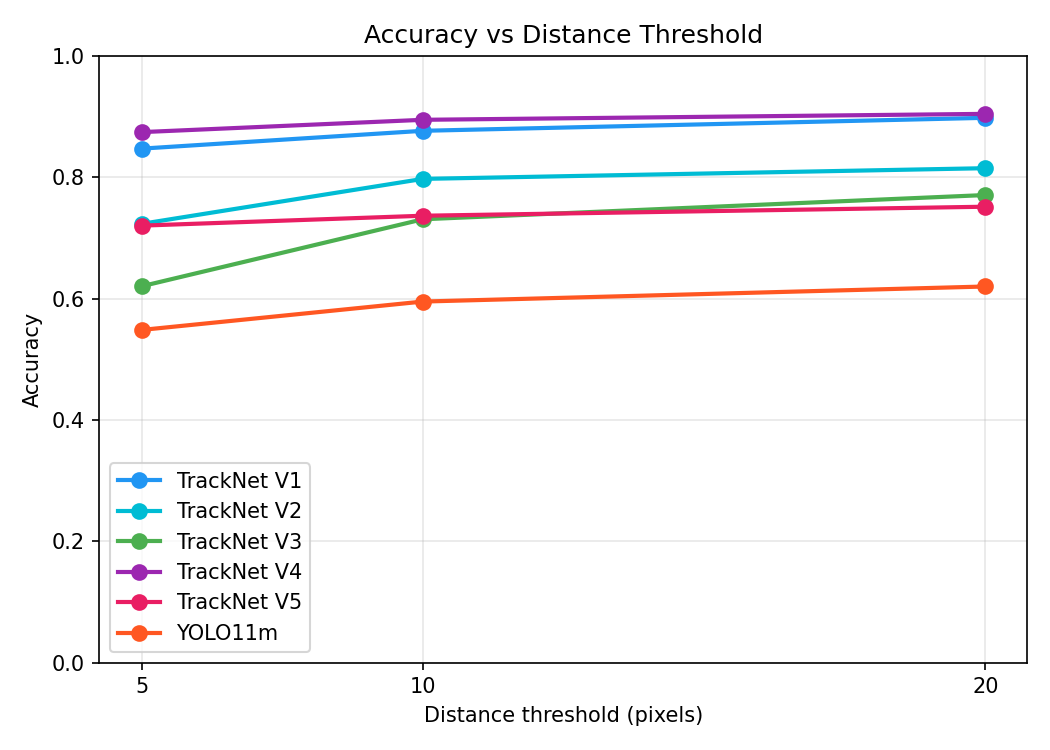
\includegraphics[width=\linewidth]{img/ball_accuracy_curves.png}
    \caption{Accuracy versus distance tolerance.}
    \label{fig:ball-acc-curves}
  \end{subfigure}\hfill
  \begin{subfigure}{0.49\textwidth}
    \centering
    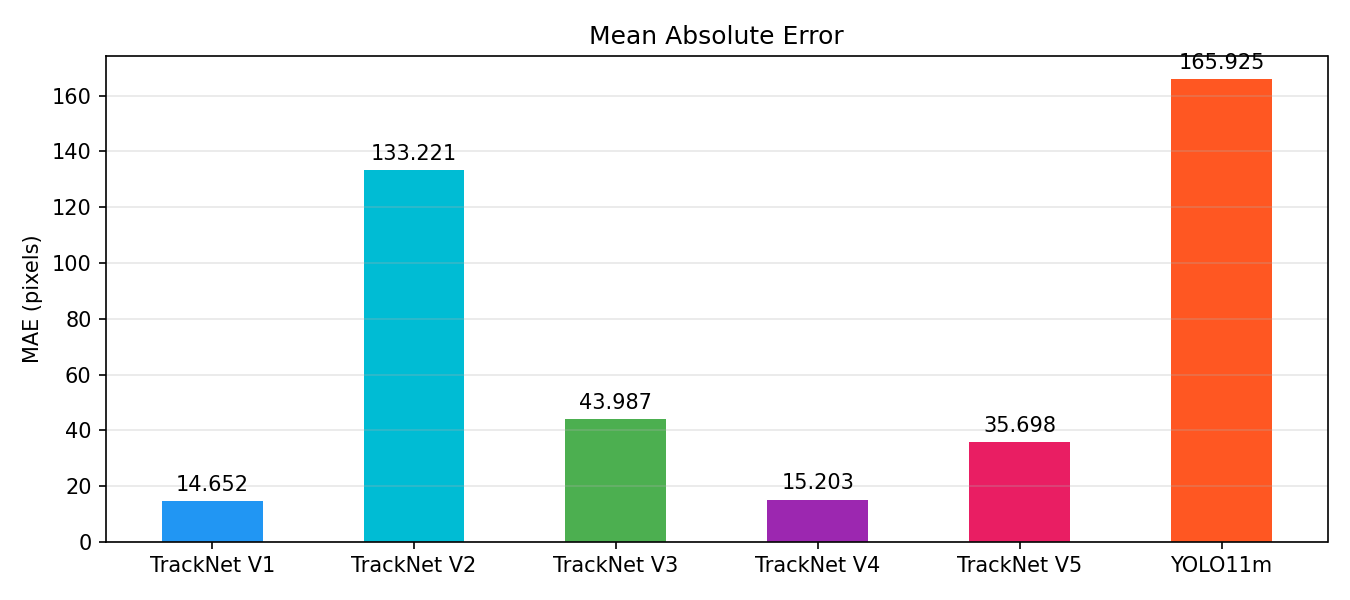
\includegraphics[width=\linewidth]{img/ball_mae_comparison.png}
    \caption{Mean absolute error.}
    \label{fig:ball-mae}
  \end{subfigure}

  \vspace{0.7em}
  \begin{subfigure}{0.49\textwidth}
    \centering
    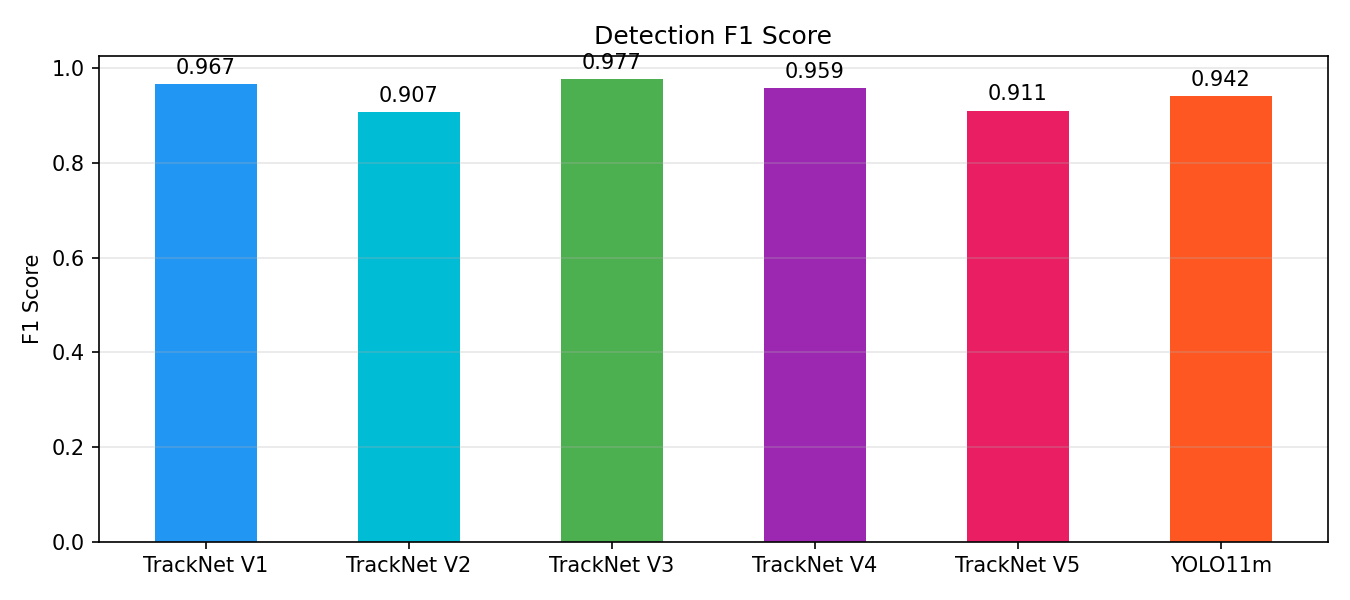
\includegraphics[width=\linewidth]{img/ball_f1_comparison.png}
    \caption{Detection $F_1$.}
    \label{fig:ball-f1}
  \end{subfigure}

  \vspace{0.7em}
  \begin{subfigure}{0.62\textwidth}
    \centering
    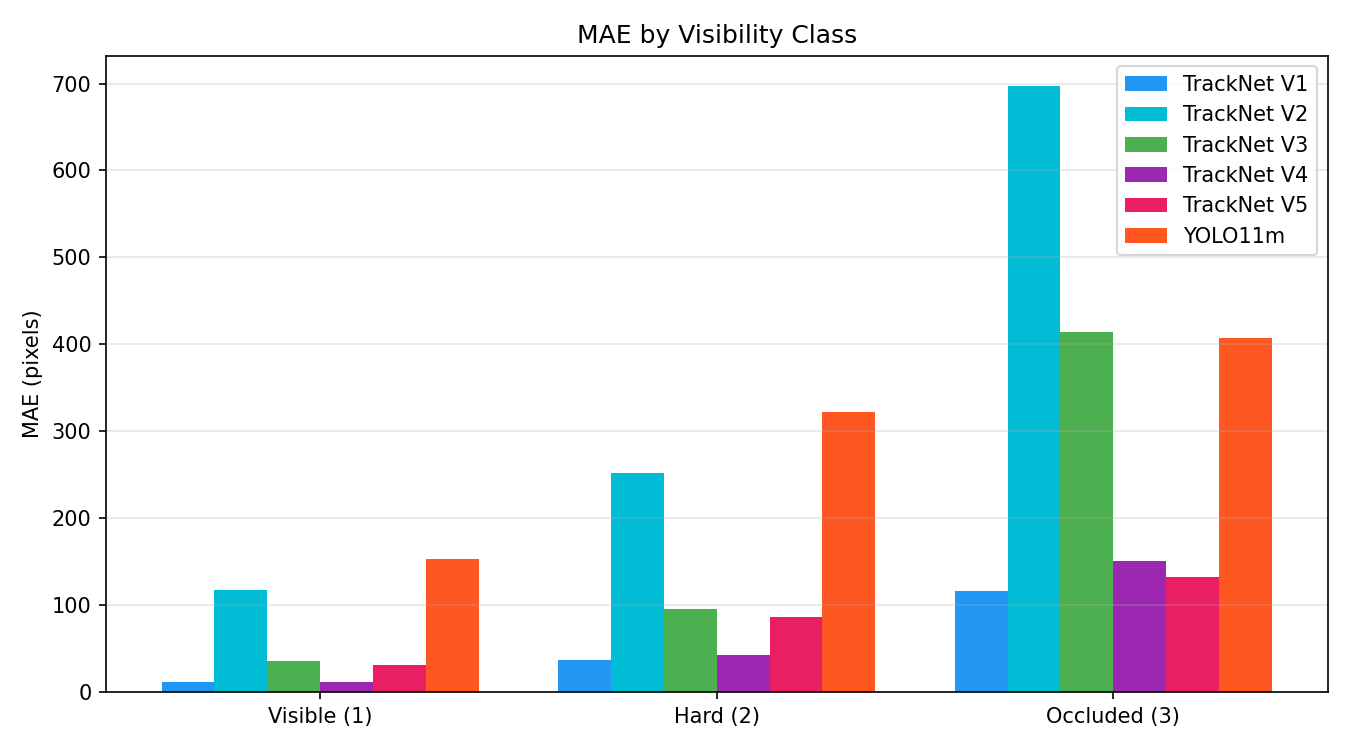
\includegraphics[width=\linewidth]{img/ball_visibility_mae.png}
    \caption{Mean absolute error by visibility class.}
    \label{fig:ball-vismae}
  \end{subfigure}

  \caption{Six-model comparison on the subset test match (game7); the plotted
    values are those tabulated in Table~\ref{tab:ball-selection}.
    (a)~Localisation accuracy across the $\{5, 10, 20\}$-pixel tolerance sweep,
    where TrackNetV4 and V1 lead while YOLO11m trails. (b)~Mean absolute error
    and (c)~detection $F_1$. (d)~Mean
    absolute error split by visibility class, showing that all models degrade
    from clearly visible to occluded balls, with the heaviest tails for V2 and
    YOLO11m.}
  \label{fig:ball-selection}
\end{figure}

\subsection{The case for TrackNetV4}
\label{sec:ball-selection-why}

TrackNetV4 was selected on three grounds. First, it is the strongest localiser
at strict tolerance: it attains the highest accuracy at all three thresholds,
and in particular the highest acc@5px (0.875), the most demanding and the most
decision-relevant of the localisation metrics for a ball whose position must
later feed a geometric line call. Second, it produces the smoothest track, with
the lowest tracking consistency of all six models (10.44 pixels), below V1's
13.98 and far below the V2, V3, and YOLO values; a steady trajectory directly
benefits the downstream bounce detector and the court projection. Third, it is
among the fastest, at 53.07 frames per second, effectively tied with the
quickest model and between two and four times the throughput of V2, V3, and V5.
TrackNetV4 therefore sits at the favourable corner of the accuracy-speed
trade-off, offering the best strict-tolerance accuracy at a negligible cost in
speed.

The remaining models were not selected for reasons that the table makes
concrete. V1 is the only genuine rival: it records a marginally lower mean error
(14.65 against 15.20 pixels), higher recall (0.966 against 0.937), and a few
more frames per second, but its acc@5px is lower and its track is noticeably
jitterier, so V4's motion attention is read as buying sharper and steadier
localisation at the strict tolerance for almost no speed penalty. V2 attains the
highest precision but its recall collapses to 0.831 and its mean error is
catastrophic at 133 pixels, indicating that it frequently fails to localise the
ball at all on this subset. V3 has the best recall and $F_1$, meaning it finds
the ball most often, yet it records the lowest acc@5px of the TrackNet family
(0.620) and the lowest throughput (13.73 frames per second): its inpainting
rectifier recovers the presence of the ball without recovering its precise
position. V5 is middling on every axis, suggesting that learned temporal
self-attention adds parameters and cost without an accuracy gain over the
explicit motion cue of V4 on this data. YOLO11m is the weakest localiser
overall, with the lowest acc@5px (0.548), a mean error of 166 pixels, and by far
the jitteriest track (74.79), which is consistent with the expectation that
box-centre regression localises a tiny ball less precisely than dense heatmap
regression.

These observations answer RQ1 directly. The progression from V1 to V5 is not
monotone in accuracy: the later variants are not uniformly better, and the
strongest strict-tolerance localiser is V4, whose motion-attention mechanism
proves to be the most effective of the temporal modules tried. The single-frame
bounding-box detector is clearly inferior to the heatmap trackers for this
target, which supports the thesis's broader claim that heatmap regression is the
more suitable formulation for a small, fast ball.

\section{Final Model's Results: TrackNetV4 on the Full Dataset}
\label{sec:ball-final}

The second stage retrained the selected model, TrackNetV4, on the full dataset
split of Section~\ref{sec:meth-splits-tracknet}: matches game1 through game9
for training and validation, and game10 held out in its entirety as the test
match. Its closest rival from the selection stage, the original TrackNet (V1),
was retrained on the identical split as a reference baseline, to test whether
the architecture ranking of Section~\ref{sec:ball-selection} survives the move
to the full dataset. Training of TrackNetV4 ran for 100 epochs and recorded a
best validation acc@5px of 0.938 at epoch~73; its loss and validation-accuracy
curves are shown in Figure~\ref{fig:ball-v4-training}. Both models were then
evaluated on the unseen game10 test match, and the resulting test metrics are
reported in Table~\ref{tab:ball-final}. These figures are the headline ball
result of the thesis; they are measured on a different and larger split than the
selection numbers of Table~\ref{tab:ball-selection} and must not be compared
column-for-column with them.

\begin{figure}[t]
  \centering
  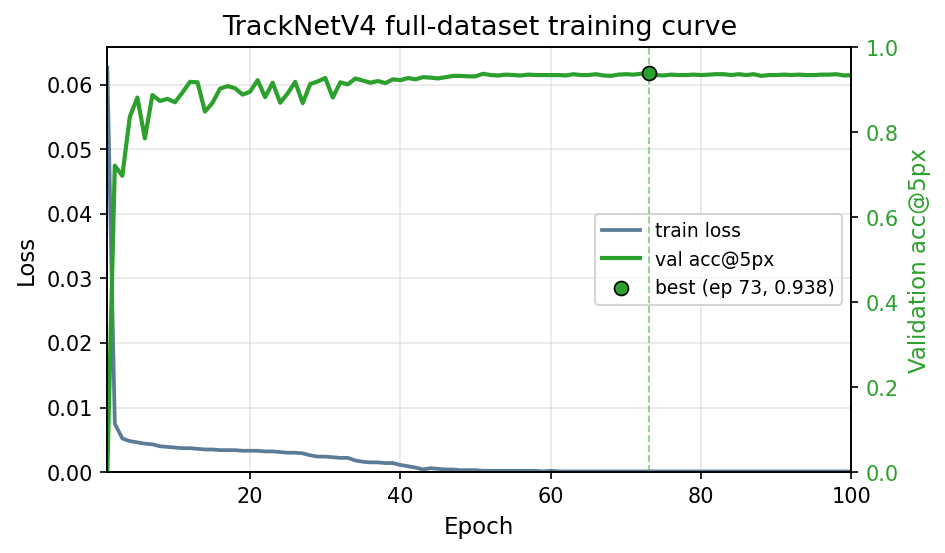
\includegraphics[width=0.8\textwidth]{img/ball_v4_training_curves.png}
  \caption{Training curve of the final TrackNetV4 on the full dataset split
    (game1--game9 for training and validation). The training loss (left axis) and
    validation accuracy at five pixels (right axis) are both plotted on linear
    scales against the epoch count. The training loss falls steeply over the first
    few epochs and then continues to decrease; validation acc@5px climbs to a plateau
    around 0.93 and peaks at 0.938 at epoch~73 (marked), the checkpoint carried
    forward for evaluation.}
  \label{fig:ball-v4-training}
\end{figure}

\begin{table}[t]
  \centering
  \footnotesize
  \setlength{\tabcolsep}{4pt}
  \caption{Final metrics of TrackNetV4 and its closest rival, the original
    TrackNet (V1), both retrained on the full dataset split and evaluated on the
    held-out test match (game10) at the best validation checkpoint. Bold marks
    the better of the two values in each column; lower is better for the MAE
    columns and tracking consistency (TC). The four MAE columns give the mean
    localisation error in pixels: overall (all) and, split by visibility class,
    for clearly visible (vis1), hard-to-identify (vis2), and occluded (vis3)
    balls. P@5px, R@5px, and $F_1$@5px are the location-aware detection metrics
    of Section~\ref{sec:meth-metrics-det}. The frames-per-second figures were
    measured on different hardware and under a different timing protocol than
    Table~\ref{tab:ball-selection} and are not comparable with that table (see
    text).}
  \label{tab:ball-final}
  \resizebox{\textwidth}{!}{%
  \begin{tabular}{l rrr rrrr rrr rrr rr}
    \toprule
    & \multicolumn{3}{c}{Localisation acc} & \multicolumn{4}{c}{MAE (px)}
    & \multicolumn{3}{c}{Detection} & \multicolumn{3}{c}{Detection @5px}
    & \multicolumn{2}{c}{} \\
    \cmidrule(lr){2-4}\cmidrule(lr){5-8}\cmidrule(lr){9-11}\cmidrule(lr){12-14}
    Model & \makecell[r]{acc@\\5px} & \makecell[r]{acc@\\10px} & \makecell[r]{acc@\\20px}
    & all & vis1 & vis2 & vis3 & Prec & Rec & $F_1$
    & \makecell[r]{P@\\5px} & \makecell[r]{R@\\5px} & \makecell[r]{$F_1$@\\5px}
    & \makecell[r]{TC} & FPS \\
    \midrule
    TrackNet (V1)       & 0.948 & 0.952 & 0.954 & 16.08 & 9.81 & 78.28 & 317.72 & \textbf{1.000} & 0.957 & 0.978 & \textbf{0.990} & 0.948 & \textbf{0.969} & \textbf{7.85} & \textbf{43.65} \\
    \textbf{TrackNetV4} & \textbf{0.956} & \textbf{0.959} & \textbf{0.963} & \textbf{12.13} & \textbf{6.89} & \textbf{63.87} & 317.72 & 0.996 & \textbf{0.972} & \textbf{0.984} & 0.980 & \textbf{0.956} & 0.968 & 8.82 & 40.82 \\
    \bottomrule
  \end{tabular}}
\end{table}

Several features of Table~\ref{tab:ball-final} deserve comment, and they are
relevant to how the numbers are quoted elsewhere in the thesis. First, the
selection-stage ranking holds on the full dataset: TrackNetV4 again leads its
closest rival V1 on strict-tolerance accuracy (acc@5px of 0.956 against 0.948)
and on mean error in every visibility class, while V1 retains the marginally
higher precision (1.000 against 0.996), the smoother track (a tracking
consistency of 7.85 against 8.82 pixels), and a few more frames per second
(43.65 against 40.82). This is the same accuracy-against-smoothness trade-off
seen at selection, now confirmed on a larger and previously unseen match, and it
justifies carrying V4 forward as the system's ball tracker. Second, the
strict-tolerance accuracy of V4 rises substantially relative to the selection
stage, from 0.875 on the subset to 0.956 on the full split, and it does so even
though the final model is scored on a finer $640 \times 368$ grid, on which five
pixels is a stricter tolerance than on the selection stage's $256 \times 256$
grid; the larger and more varied training set, together with the higher
resolution, sharpens localisation on clearly visible balls. The two stages' mean
errors are measured on these different grids and so are not directly comparable
in raw pixels, but the final aggregate of 12.13 pixels for V4 is dominated, as at
selection, by a heavy tail of difficult cases: on clearly visible balls
(visibility class~1) the mean error is tight at 6.89 pixels, whereas on the rare
hard-to-identify balls (class~2) it is 63.87 pixels and on the still rarer
occluded balls (class~3) it is 317.72 pixels. For this reason acc@5px, and not
the mean error, is quoted as the headline localisation figure throughout. The
track remains smooth, with a tracking consistency of 8.82 pixels, and precision
is near-perfect at 0.996 on game10, so that almost every reported ball is a true
positive, while the location-aware $F_1$@5px of 0.968 confirms that the great
majority of detections are also well localised.


\section{Analysis}
\label{sec:ball-analysis}

The selection result and the final metrics together support a coherent picture
of why TrackNetV4 succeeds and where it remains limited. Its advantage traces to
the motion-attention module: by gating the decoder with a map of inter-frame
motion, the network concentrates its capacity on the regions where a fast ball
actually appears, which sharpens the response peak and, as the tracking
consistency shows, steadies the trajectory between frames. This is achieved at
essentially no parameter cost over the V1 backbone, which is why V4 dominates V1
on strict-tolerance accuracy and smoothness while matching it on speed. The
comparison with V5 is instructive in the same vein: the explicit, almost
free motion cue of V4 outperformed the heavier learned temporal self-attention
of V5 on this data, indicating that for this target a strong inductive bias
towards motion is more effective than a general attention mechanism left to
learn the same cue.

The per-visibility breakdown locates the residual difficulty precisely. The
model is accurate when the ball is clearly visible, which is the common case,
but its error grows by an order of magnitude on the motion-blurred and occluded
frames of visibility classes~2 and~3. Figure~\ref{fig:ball-final-overlay} shows
the final model's output on four frames sampled across a held-out game10 rally,
where the predicted ball position (red) tracks the ground truth (green) to
within a few pixels throughout. The dominant failure modes are the ones
that the task formulation anticipates: a ball occluded by a player or the net,
which leaves no peak for the heatmap to find; a ball moving fast enough to blur
across many pixels, which broadens and weakens the response; and a ball near or
beyond the frame edge, which has no well-defined centre. These cases are rare in
the dataset and are reflected in the heavy tail of the mean error rather than in
the strict-tolerance accuracy, but they are the natural targets for the future
work discussed in Chapter~\ref{ch:conclusion}, and they are precisely the
situations in which the downstream trajectory rectification and event detection
must be robust.

\begin{figure}[tbp]
  \centering
  \begin{subfigure}{0.49\textwidth}
    \centering
    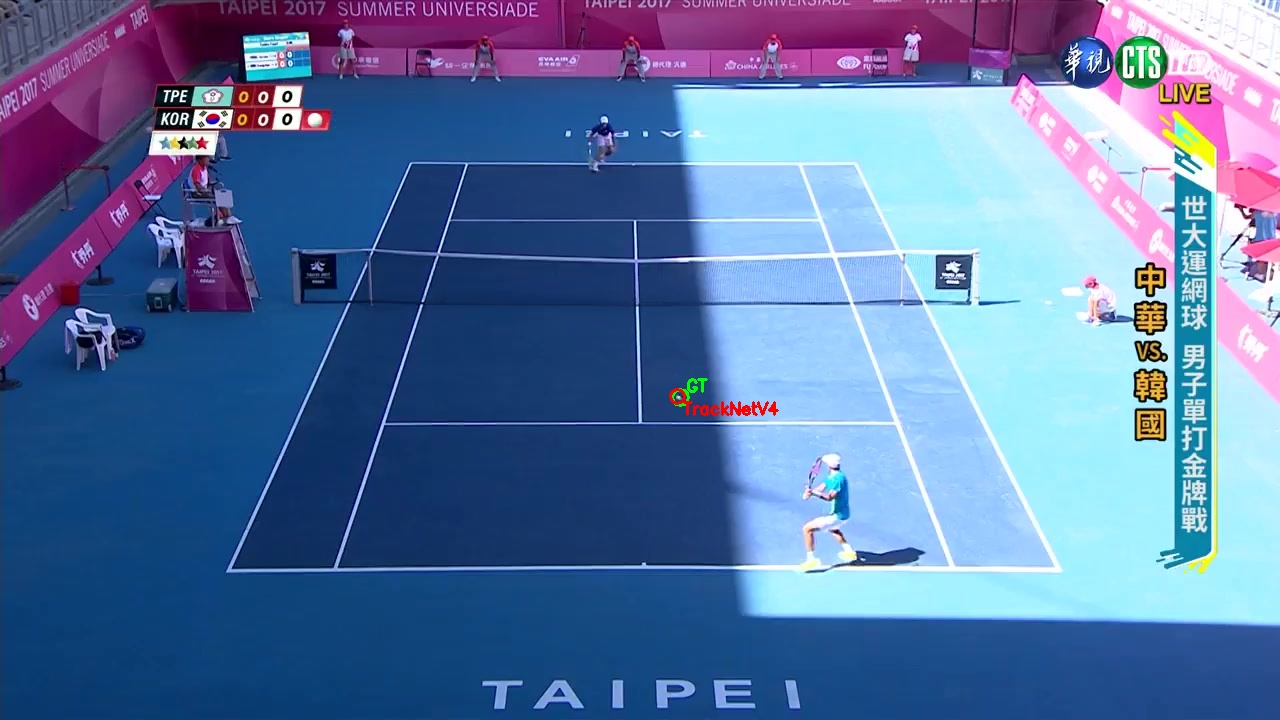
\includegraphics[width=\linewidth]{img/ball_overlay_frame001.jpg}
    \caption{Frame 1.}
    \label{fig:ball-overlay-f1}
  \end{subfigure}\hfill
  \begin{subfigure}{0.49\textwidth}
    \centering
    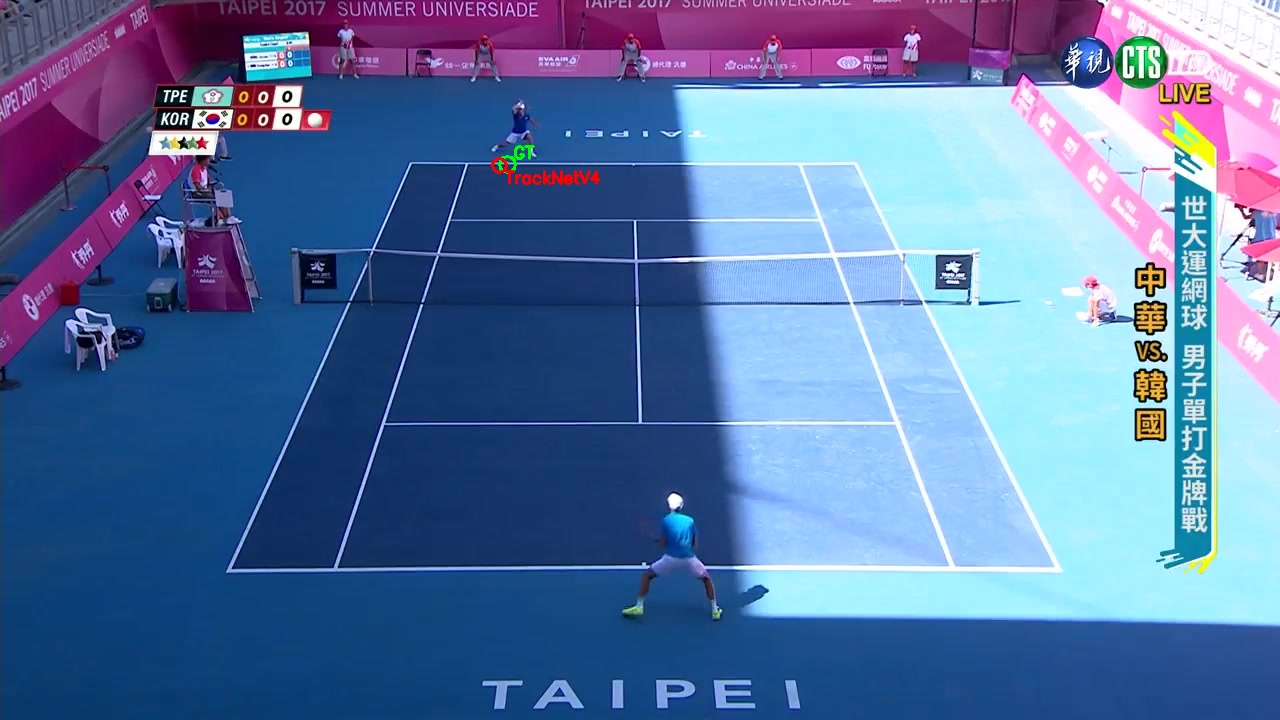
\includegraphics[width=\linewidth]{img/ball_overlay_frame050.jpg}
    \caption{Frame 50 (visibility class~2).}
    \label{fig:ball-overlay-f2}
  \end{subfigure}

  \vspace{0.5em}
  \begin{subfigure}{0.49\textwidth}
    \centering
    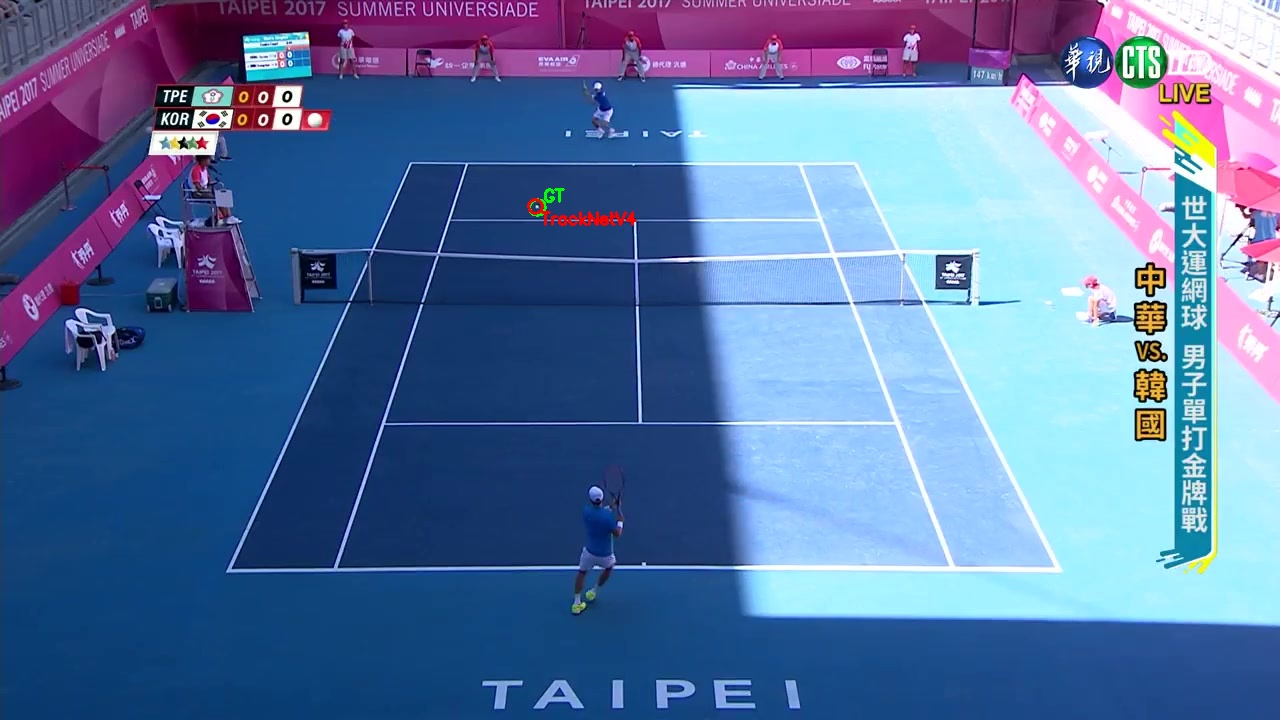
\includegraphics[width=\linewidth]{img/ball_overlay_frame100.jpg}
    \caption{Frame 100.}
    \label{fig:ball-overlay-f3}
  \end{subfigure}\hfill
  \begin{subfigure}{0.49\textwidth}
    \centering
    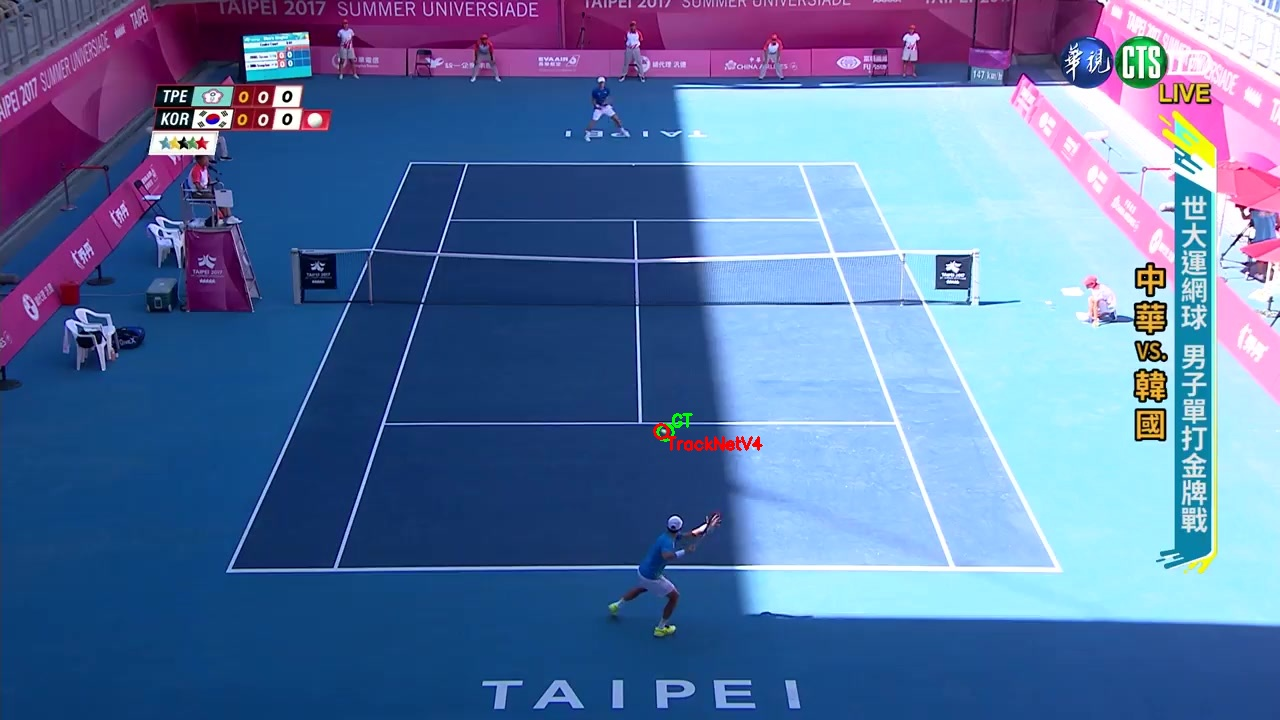
\includegraphics[width=\linewidth]{img/ball_overlay_frame150.jpg}
    \caption{Frame 150.}
    \label{fig:ball-overlay-f4}
  \end{subfigure}
  \caption{Qualitative output of the final TrackNetV4 model on four frames
    sampled across a held-out game10 rally. In each frame the ground-truth ball
    position (green, GT) and the model's prediction (red, TrackNetV4) are
    overlaid; the two markers coincide to within a few pixels throughout,
    including the motion-blurred mid-court frame of visibility class~2~(b). The
    ball is localised accurately across the full range of court positions and
    play phases seen in the rally.}
  \label{fig:ball-final-overlay}
\end{figure}

In summary, the two-stage comparison answers RQ1 by identifying TrackNetV4 as
the best ball-tracking model among the six considered, on the grounds of
strict-tolerance accuracy and trajectory smoothness at competitive speed, and by
showing that the architectural progression through the family is not monotone
and that the heatmap formulation is clearly preferable to single-frame
bounding-box detection for this target. The selected model carries forward to
the integrated system of Chapter~\ref{ch:integrated} as the ball-tracking
component, where its smooth, well-localised trajectory feeds the bounce detector
of Chapter~\ref{ch:bounce} and the court projection of Chapter~\ref{ch:court}.
